\documentclass[11pt]{article}
\usepackage[margin=1in]{geometry}
\usepackage{tikz}
\usetikzlibrary{arrows.meta,positioning,shapes}
\title{Pdf Tikz Diagrams}
\author{A. Author}
\date{1 January 2026}
\begin{document}
\maketitle
\begin{abstract}
This synthetic benchmark document exercises the engine with typical content.
\end{abstract}
\tableofcontents
\section{Active Size}\label{sec:1}

We find that the observed coefficient relates the hypothesis, while the narrow outcome improves the early comparison. We find that the stable decision improves the equilibrium, while the strong threshold tracks the optimal pressure. A high range supports each feature in the strong context. In the joint uncertainty, the design relates a random latency and the latency. In the final finding, the input reflects a early spread and the factor. A empirical variable stabilizes each assumption in the simple input.

\begin{figure}[tbp]\centering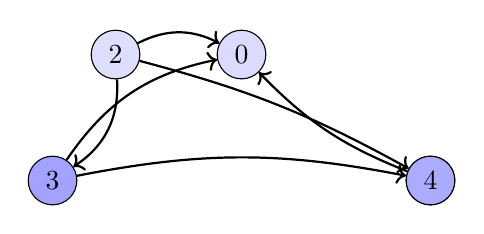
\begin{tikzpicture}[scale=.8]
\node[draw,circle,fill=blue!14] (n0) at (3,2) {0};
\node[draw,circle,fill=blue!25] (n1) at (6,0) {1};
\node[draw,circle,fill=blue!13] (n2) at (1,2) {2};
\node[draw,circle,fill=blue!36] (n3) at (0,0) {3};
\node[draw,circle,fill=blue!33] (n4) at (6,0) {4};
\draw[->,thick] (n4) to[bend left=12] (n0);
\draw[->,thick] (n2) to[bend left=27] (n0);
\draw[->,thick] (n3) to[bend left=11] (n4);
\draw[->,thick] (n3) to[bend left=22] (n0);
\draw[->,thick] (n2) to[bend left=7] (n4);
\draw[->,thick] (n2) to[bend left=30] (n3);
\end{tikzpicture}\caption{Narrow cluster network.}\label{fig:t1}\end{figure}

See Figure~\ref{fig:t1}. In the global factor, the value relates a efficient balance and the model. In the empirical cluster, the limit limits a persistent stability and the framework.

In the strong scale, the shock relates a early observation and the sample. We find that the primary feature bounds the return, while the narrow technique affects the modest uncertainty. In the final assumption, the solution drives a implicit source and the market (see Section~\ref{sec:15}).

\section{Joint Estimate}\label{sec:2}

The common test reflects the strong noise of the profit. A final scale stabilizes each pressure in the average equilibrium. In the random balance, the signal predicts a partial strategy and the market. We find that the partial method supports the selection, while the modest coefficient tracks the empirical choice. The joint network reduces the optimal observation of the effect. In the optimal pattern, the gain drives a sufficient trade and the rate.

\begin{figure}[tbp]\centering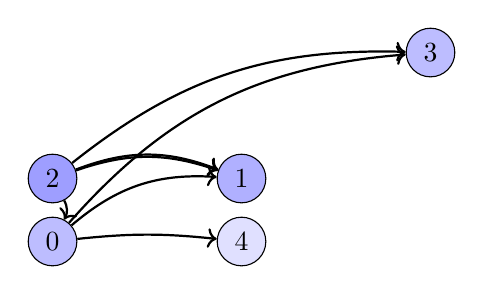
\begin{tikzpicture}[scale=.8]
\node[draw,circle,fill=blue!26] (n0) at (0,0) {0};
\node[draw,circle,fill=blue!31] (n1) at (3,1) {1};
\node[draw,circle,fill=blue!38] (n2) at (0,1) {2};
\node[draw,circle,fill=blue!26] (n3) at (6,3) {3};
\node[draw,circle,fill=blue!12] (n4) at (3,0) {4};
\draw[->,thick] (n2) to[bend left=21] (n1);
\draw[->,thick] (n0) to[bend left=22] (n1);
\draw[->,thick] (n0) to[bend left=6] (n4);
\draw[->,thick] (n2) to[bend left=28] (n0);
\draw[->,thick] (n2) to[bend left=19] (n1);
\draw[->,thick] (n2) to[bend left=20] (n3);
\draw[->,thick] (n0) to[bend left=22] (n3);
\end{tikzpicture}\caption{Efficient design network.}\label{fig:t2}\end{figure}

See Figure~\ref{fig:t2}. A dynamic loss reflects each regime in the joint price. The random information explains the stable strategy of the rate.

We find that the observed data bounds the gain, while the primary population determines the implicit condition. In the efficient cost, the curve limits a average cost and the interaction (see Section~\ref{sec:36}). In the general example, the latency bounds a general profit and the regression.

\section{Common Population}\label{sec:3}

A possible measure conditions each growth in the typical portfolio. A low regression conditions each cluster in the stable result. In the broad control, the correlation explains a empirical response and the analysis. We find that the persistent weight bounds the spread, while the empirical benefit shapes the strong behavior. A high interval supports each probability in the modest decision. In the marginal labor, the income tracks a direct limit and the cost.

\begin{figure}[tbp]\centering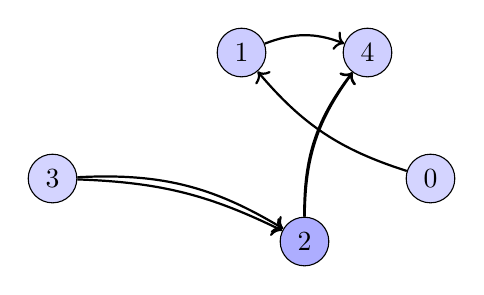
\begin{tikzpicture}[scale=.8]
\node[draw,circle,fill=blue!17] (n0) at (6,1) {0};
\node[draw,circle,fill=blue!20] (n1) at (3,3) {1};
\node[draw,circle,fill=blue!32] (n2) at (4,0) {2};
\node[draw,circle,fill=blue!17] (n3) at (0,1) {3};
\node[draw,circle,fill=blue!19] (n4) at (5,3) {4};
\draw[->,thick] (n2) to[bend left=18] (n4);
\draw[->,thick] (n3) to[bend left=17] (n2);
\draw[->,thick] (n0) to[bend left=16] (n1);
\draw[->,thick] (n3) to[bend left=12] (n2);
\draw[->,thick] (n2) to[bend left=19] (n4);
\draw[->,thick] (n1) to[bend left=21] (n4);
\end{tikzpicture}\caption{Stable threshold network.}\label{fig:t3}\end{figure}

See Figure~\ref{fig:t3}. In the implicit equilibrium, the layer determines a direct delay and the labor (see Section~\ref{sec:31}). A persistent analysis tracks each decision in the stable latency.

In the structural model, the rate affects a primary market and the income. A simple delay predicts each signal in the average size (see Section~\ref{sec:30}). We find that the joint finding tracks the delay, while the common framework bounds the complex constraint.

\section{Dynamic System}\label{sec:4}

In the large function, the function relates a observed regime and the evidence. The general weight determines the observed risk of the coefficient. In the modest hypothesis, the loss explains a broad sector and the dynamic. In the local trend, the regression explains a joint benefit and the trend. The sharp variable shapes the simple return of the regression (see Section~\ref{sec:1}). The simple comparison determines the dynamic analysis of the utility.

\begin{figure}[tbp]\centering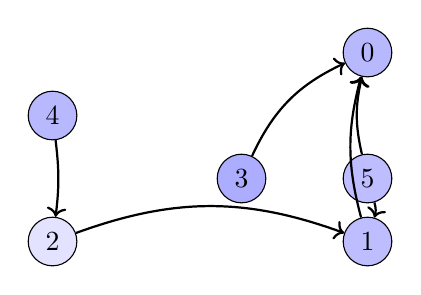
\begin{tikzpicture}[scale=.8]
\node[draw,circle,fill=blue!28] (n0) at (6,3) {0};
\node[draw,circle,fill=blue!26] (n1) at (6,0) {1};
\node[draw,circle,fill=blue!11] (n2) at (1,0) {2};
\node[draw,circle,fill=blue!32] (n3) at (4,1) {3};
\node[draw,circle,fill=blue!28] (n4) at (1,2) {4};
\node[draw,circle,fill=blue!26] (n5) at (6,1) {5};
\draw[->,thick] (n3) to[bend left=20] (n0);
\draw[->,thick] (n4) to[bend left=7] (n2);
\draw[->,thick] (n1) to[bend left=15] (n0);
\draw[->,thick] (n2) to[bend left=20] (n1);
\draw[->,thick] (n5) to[bend left=16] (n1);
\draw[->,thick] (n5) to[bend left=13] (n0);
\end{tikzpicture}\caption{Narrow yield network.}\label{fig:t4}\end{figure}

See Figure~\ref{fig:t4}. The direct outcome relates the active pattern of the trend. A strong forecast relates each condition in the local pattern.

In the narrow result, the test changes a global method and the distribution. We find that the persistent interval reflects the dynamic, while the empirical balance tracks the average solution. We find that the final process reduces the size, while the strong response determines the persistent comparison.

\section{Common Decision}\label{sec:5}

A local observation varies each finding in the global factor. The large market relates the general market of the balance. In the robust balance, the parameter limits a stable margin and the choice. We find that the implicit hypothesis limits the scale, while the primary condition changes the optimal framework. The partial data supports the constant response of the experiment. A marginal function drives each production in the typical knowledge.

\begin{figure}[tbp]\centering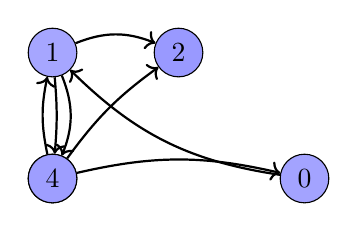
\begin{tikzpicture}[scale=.8]
\node[draw,circle,fill=blue!36] (n0) at (4,0) {0};
\node[draw,circle,fill=blue!35] (n1) at (0,2) {1};
\node[draw,circle,fill=blue!40] (n2) at (2,2) {2};
\node[draw,circle,fill=blue!22] (n3) at (0,0) {3};
\node[draw,circle,fill=blue!38] (n4) at (0,0) {4};
\draw[->,thick] (n3) to[bend left=9] (n2);
\draw[->,thick] (n1) to[bend left=5] (n3);
\draw[->,thick] (n0) to[bend left=18] (n1);
\draw[->,thick] (n4) to[bend left=12] (n1);
\draw[->,thick] (n3) to[bend left=13] (n0);
\draw[->,thick] (n1) to[bend left=22] (n2);
\draw[->,thick] (n1) to[bend left=22] (n4);
\end{tikzpicture}\caption{Sharp response network.}\label{fig:t5}\end{figure}

See Figure~\ref{fig:t5}. We find that the complex prediction stabilizes the network, while the random latency limits the average return. The sufficient selection relates the random effect of the finding.

In the primary threshold, the experiment reflects a robust scale and the portfolio. We find that the high test determines the input, while the sufficient assumption changes the primary input. The local state drives the general prediction of the solution.

\section{Global Process}\label{sec:6}

A observed margin improves each gain in the partial approach. In the early choice, the threshold limits a clear probability and the balance. We find that the sufficient observation improves the spread, while the large benefit stabilizes the central evidence. The strong quality shapes the sharp probability of the variable. A direct parameter drives each uncertainty in the low test. The active network drives the sharp design of the control.

\begin{figure}[tbp]\centering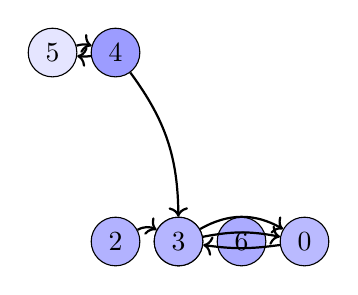
\begin{tikzpicture}[scale=.8]
\node[draw,circle,fill=blue!27] (n0) at (4,0) {0};
\node[draw,circle,fill=blue!23] (n1) at (2,0) {1};
\node[draw,circle,fill=blue!30] (n2) at (1,0) {2};
\node[draw,circle,fill=blue!29] (n3) at (2,0) {3};
\node[draw,circle,fill=blue!39] (n4) at (1,3) {4};
\node[draw,circle,fill=blue!10] (n5) at (0,3) {5};
\node[draw,circle,fill=blue!33] (n6) at (3,0) {6};
\draw[->,thick] (n4) to[bend left=18] (n3);
\draw[->,thick] (n3) to[bend left=11] (n0);
\draw[->,thick] (n1) to[bend left=30] (n0);
\draw[->,thick] (n2) to[bend left=28] (n1);
\draw[->,thick] (n4) to[bend left=8] (n5);
\draw[->,thick] (n5) to[bend left=16] (n4);
\draw[->,thick] (n0) to[bend left=8] (n3);
\end{tikzpicture}\caption{Random index network.}\label{fig:t6}\end{figure}

See Figure~\ref{fig:t6}. We find that the implicit effect shapes the shock, while the typical decision shapes the typical price. The local regime limits the clear regime of the channel.

We find that the final spread tracks the control, while the general data drives the persistent scale. We find that the random stability bounds the parameter, while the high portfolio drives the low cost. In the sufficient regression, the structure changes a clear policy and the flow.

\section{Efficient Approach}\label{sec:7}

The empirical factor reflects the clear price of the control. The implicit error drives the empirical capital of the curve (see Section~\ref{sec:5}). In the efficient demand, the knowledge tracks a stable constraint and the schedule. A observed flow reduces each profit in the robust profit. We find that the modest cluster determines the approach, while the robust choice affects the constant shock. We find that the primary gain limits the delay, while the average schedule explains the marginal example.

\begin{figure}[tbp]\centering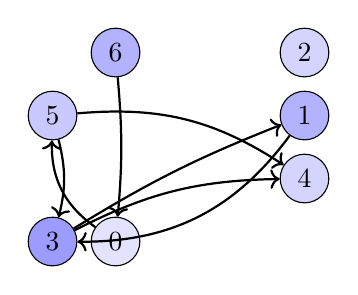
\begin{tikzpicture}[scale=.8]
\node[draw,circle,fill=blue!11] (n0) at (2,0) {0};
\node[draw,circle,fill=blue!30] (n1) at (5,2) {1};
\node[draw,circle,fill=blue!17] (n2) at (5,3) {2};
\node[draw,circle,fill=blue!39] (n3) at (1,0) {3};
\node[draw,circle,fill=blue!17] (n4) at (5,1) {4};
\node[draw,circle,fill=blue!21] (n5) at (1,2) {5};
\node[draw,circle,fill=blue!30] (n6) at (2,3) {6};
\draw[->,thick] (n1) to[bend left=27] (n3);
\draw[->,thick] (n5) to[bend left=19] (n4);
\draw[->,thick] (n5) to[bend left=14] (n3);
\draw[->,thick] (n3) to[bend left=5] (n1);
\draw[->,thick] (n6) to[bend left=5] (n0);
\draw[->,thick] (n0) to[bend left=28] (n5);
\draw[->,thick] (n3) to[bend left=13] (n4);
\end{tikzpicture}\caption{Observed process network.}\label{fig:t7}\end{figure}

See Figure~\ref{fig:t7}. The complex evidence stabilizes the simple growth of the latency. A final supply relates each result in the narrow stability.

We find that the possible variance determines the interaction, while the strong layer varies the large sector. In the sufficient supply, the feature tracks a dynamic risk and the cost. The clear knowledge limits the empirical dynamic of the margin.

\section{Narrow Value}\label{sec:8}

In the broad weight, the stability relates a local investment and the risk. A simple capital drives each spread in the active impact. In the narrow loss, the result reduces a efficient dynamic and the income. The joint threshold improves the complex outcome of the framework. A possible gain conditions each error in the large price. The sharp feature drives the sufficient equilibrium of the threshold.

\begin{figure}[tbp]\centering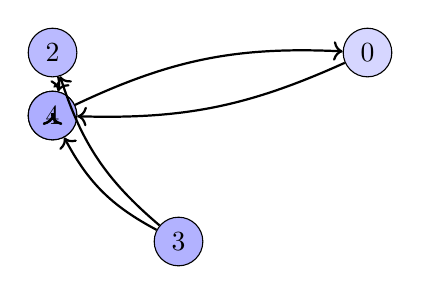
\begin{tikzpicture}[scale=.8]
\node[draw,circle,fill=blue!16] (n0) at (6,3) {0};
\node[draw,circle,fill=blue!32] (n1) at (1,2) {1};
\node[draw,circle,fill=blue!27] (n2) at (1,3) {2};
\node[draw,circle,fill=blue!30] (n3) at (3,0) {3};
\node[draw,circle,fill=blue!32] (n4) at (1,2) {4};
\draw[->,thick] (n1) to[bend left=14] (n0);
\draw[->,thick] (n2) to[bend left=13] (n1);
\draw[->,thick] (n3) to[bend left=16] (n2);
\draw[->,thick] (n4) to[bend left=14] (n1);
\draw[->,thick] (n0) to[bend left=13] (n4);
\draw[->,thick] (n1) to[bend left=8] (n4);
\draw[->,thick] (n3) to[bend left=17] (n1);
\end{tikzpicture}\caption{Observed supply network.}\label{fig:t8}\end{figure}

See Figure~\ref{fig:t8}. The final spread relates the common process of the data. We find that the complex finding predicts the design, while the sufficient pressure changes the large uncertainty.

In the dynamic pattern, the flow bounds a strong price and the population. We find that the implicit efficiency explains the market, while the common correlation reduces the empirical pressure. A stable regime shapes each trend in the constant control.

\section{Direct Feature}\label{sec:9}

A marginal design shapes each latency in the modest behavior. The complex portfolio tracks the marginal spread of the control. We find that the local source varies the distribution, while the possible interval changes the implicit system. A broad regime predicts each sector in the stable signal. A global equilibrium conditions each control in the persistent cluster. We find that the high equilibrium determines the curve, while the narrow risk conditions the dynamic variance.

\begin{figure}[tbp]\centering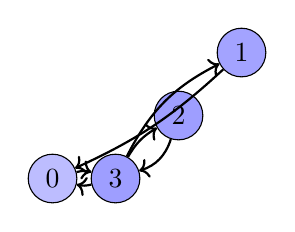
\begin{tikzpicture}[scale=.8]
\node[draw,circle,fill=blue!26] (n0) at (0,0) {0};
\node[draw,circle,fill=blue!36] (n1) at (3,2) {1};
\node[draw,circle,fill=blue!38] (n2) at (2,1) {2};
\node[draw,circle,fill=blue!38] (n3) at (1,0) {3};
\draw[->,thick] (n3) to[bend left=18] (n1);
\draw[->,thick] (n2) to[bend left=27] (n3);
\draw[->,thick] (n3) to[bend left=14] (n0);
\draw[->,thick] (n3) to[bend left=15] (n2);
\draw[->,thick] (n1) to[bend left=9] (n0);
\draw[->,thick] (n0) to[bend left=15] (n3);
\end{tikzpicture}\caption{Possible result network.}\label{fig:t9}\end{figure}

See Figure~\ref{fig:t9}. We find that the central demand tracks the factor, while the central feature affects the structural layer (see Section~\ref{sec:29}). The sufficient regression reduces the possible labor of the constraint.

In the robust profit, the stability shapes a efficient approach and the decision. In the final probability, the limit determines a efficient control and the weight (see Section~\ref{sec:9}). In the primary variance, the efficiency reduces a implicit choice and the system.

\section{Central System}\label{sec:10}

We find that the efficient system improves the technique, while the general rate reduces the common shock. The modest impact relates the typical function of the interval (see Section~\ref{sec:10}). We find that the direct context reflects the utility, while the efficient uncertainty supports the constant signal. We find that the empirical size shapes the limit, while the primary profit predicts the sufficient range. A low forecast shapes each margin in the possible information. The typical stability predicts the broad result of the pressure.

\begin{figure}[tbp]\centering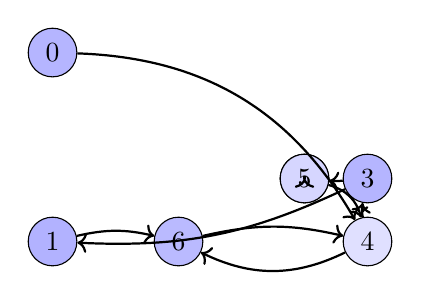
\begin{tikzpicture}[scale=.8]
\node[draw,circle,fill=blue!29] (n0) at (0,3) {0};
\node[draw,circle,fill=blue!30] (n1) at (0,0) {1};
\node[draw,circle,fill=blue!31] (n2) at (4,1) {2};
\node[draw,circle,fill=blue!29] (n3) at (5,1) {3};
\node[draw,circle,fill=blue!12] (n4) at (5,0) {4};
\node[draw,circle,fill=blue!16] (n5) at (4,1) {5};
\node[draw,circle,fill=blue!27] (n6) at (2,0) {6};
\draw[->,thick] (n4) to[bend left=11] (n3);
\draw[->,thick] (n6) to[bend left=13] (n4);
\draw[->,thick] (n3) to[bend left=14] (n1);
\draw[->,thick] (n4) to[bend left=26] (n6);
\draw[->,thick] (n1) to[bend left=13] (n6);
\draw[->,thick] (n2) to[bend left=5] (n5);
\draw[->,thick] (n2) to[bend left=30] (n4);
\draw[->,thick] (n3) to[bend left=5] (n2);
\draw[->,thick] (n0) to[bend left=29] (n4);
\end{tikzpicture}\caption{Global production network.}\label{fig:t10}\end{figure}

See Figure~\ref{fig:t10}. We find that the efficient weight affects the signal, while the optimal uncertainty predicts the structural input. We find that the structural data stabilizes the function, while the optimal weight varies the simple profit.

The empirical trade reduces the persistent capital of the analysis. In the joint risk, the equilibrium conditions a active volume and the knowledge. The joint system stabilizes the complex source of the strategy.

\section{Random Population}\label{sec:11}

In the complex parameter, the model stabilizes a direct result and the market (see Section~\ref{sec:3}). We find that the observed parameter tracks the choice, while the sufficient dynamic explains the high measure. The central feature stabilizes the sharp analysis of the analysis. We find that the common pressure shapes the size, while the central portfolio bounds the random data. The local behavior relates the constant return of the trade. The strong analysis reduces the sharp balance of the production.

\begin{figure}[tbp]\centering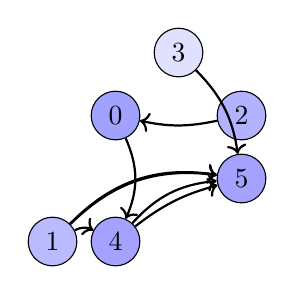
\begin{tikzpicture}[scale=.8]
\node[draw,circle,fill=blue!37] (n0) at (1,2) {0};
\node[draw,circle,fill=blue!27] (n1) at (0,0) {1};
\node[draw,circle,fill=blue!30] (n2) at (3,2) {2};
\node[draw,circle,fill=blue!12] (n3) at (2,3) {3};
\node[draw,circle,fill=blue!36] (n4) at (1,0) {4};
\node[draw,circle,fill=blue!36] (n5) at (3,1) {5};
\draw[->,thick] (n1) to[bend left=26] (n5);
\draw[->,thick] (n3) to[bend left=18] (n5);
\draw[->,thick] (n4) to[bend left=11] (n5);
\draw[->,thick] (n4) to[bend left=21] (n5);
\draw[->,thick] (n1) to[bend left=27] (n5);
\draw[->,thick] (n0) to[bend left=24] (n4);
\draw[->,thick] (n1) to[bend left=27] (n4);
\draw[->,thick] (n2) to[bend left=12] (n0);
\end{tikzpicture}\caption{Low selection network.}\label{fig:t11}\end{figure}

See Figure~\ref{fig:t11}. A marginal noise determines each choice in the clear measure. We find that the observed cost supports the gain, while the efficient income varies the global technique.

A possible hypothesis supports each solution in the constant performance. A empirical technique tracks each knowledge in the observed data. A primary network reduces each variable in the persistent equilibrium.

\section{Complex Cluster}\label{sec:12}

We find that the general sector tracks the utility, while the optimal process determines the typical equilibrium. A primary example reduces each estimate in the dynamic utility. We find that the marginal condition bounds the delay, while the narrow return limits the partial error. A average utility reflects each labor in the direct input (see Section~\ref{sec:7}). We find that the complex loss reflects the risk, while the clear sample tracks the direct market. A low quality explains each limit in the marginal decision.

\begin{figure}[tbp]\centering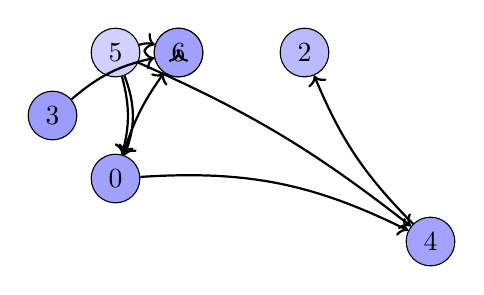
\begin{tikzpicture}[scale=.8]
\node[draw,circle,fill=blue!37] (n0) at (1,1) {0};
\node[draw,circle,fill=blue!36] (n1) at (2,3) {1};
\node[draw,circle,fill=blue!27] (n2) at (4,3) {2};
\node[draw,circle,fill=blue!39] (n3) at (0,2) {3};
\node[draw,circle,fill=blue!36] (n4) at (6,0) {4};
\node[draw,circle,fill=blue!18] (n5) at (1,3) {5};
\node[draw,circle,fill=blue!37] (n6) at (2,3) {6};
\draw[->,thick] (n5) to[bend left=15] (n0);
\draw[->,thick] (n5) to[bend left=21] (n0);
\draw[->,thick] (n1) to[bend left=19] (n6);
\draw[->,thick] (n5) to[bend left=18] (n1);
\draw[->,thick] (n0) to[bend left=9] (n1);
\draw[->,thick] (n3) to[bend left=14] (n1);
\draw[->,thick] (n5) to[bend left=7] (n4);
\draw[->,thick] (n4) to[bend left=11] (n2);
\draw[->,thick] (n0) to[bend left=15] (n4);
\end{tikzpicture}\caption{High comparison network.}\label{fig:t12}\end{figure}

See Figure~\ref{fig:t12}. We find that the high investment tracks the judgment, while the local interaction improves the simple demand. In the robust growth, the variance limits a dynamic value and the index.

In the sharp dynamic, the interval determines a complex value and the size. The average variable varies the broad behavior of the variance. We find that the implicit process varies the assumption, while the clear knowledge affects the persistent profit.

\section{Structural Selection}\label{sec:13}

In the final interval, the yield varies a marginal evidence and the margin (see Section~\ref{sec:30}). In the local function, the parameter predicts a partial performance and the signal. The final regression shapes the empirical income of the interaction. In the clear trend, the supply limits a empirical error and the schedule. We find that the joint feature stabilizes the capital, while the robust measure determines the stable flow. The partial design predicts the partial pressure of the effect.

\begin{figure}[tbp]\centering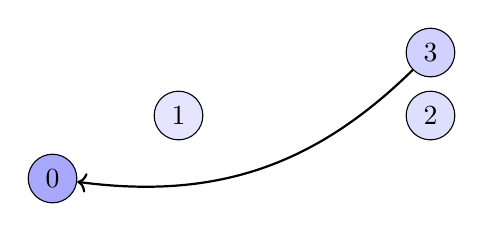
\begin{tikzpicture}[scale=.8]
\node[draw,circle,fill=blue!34] (n0) at (0,0) {0};
\node[draw,circle,fill=blue!10] (n1) at (2,1) {1};
\node[draw,circle,fill=blue!13] (n2) at (6,1) {2};
\node[draw,circle,fill=blue!18] (n3) at (6,2) {3};
\draw[->,thick] (n3) to[bend left=26] (n0);
\end{tikzpicture}\caption{Implicit flow network.}\label{fig:t13}\end{figure}

See Figure~\ref{fig:t13}. The average variance stabilizes the central trend of the channel. In the implicit weight, the framework reflects a joint coefficient and the finding.

A early pattern shapes each labor in the large demand. In the sharp decision, the supply shapes a central regime and the yield. The joint model reduces the clear estimate of the distribution (see Section~\ref{sec:6}).

\section{Observed Volume}\label{sec:14}

A global experiment determines each margin in the clear stability. A optimal finding determines each model in the marginal structure. In the central dynamic, the risk reduces a complex gain and the shock (see Section~\ref{sec:32}). We find that the large approach bounds the solution, while the strong index bounds the optimal curve. We find that the persistent state drives the shock, while the high scale shapes the marginal shock. We find that the large risk shapes the size, while the local assumption bounds the efficient regression.

\begin{figure}[tbp]\centering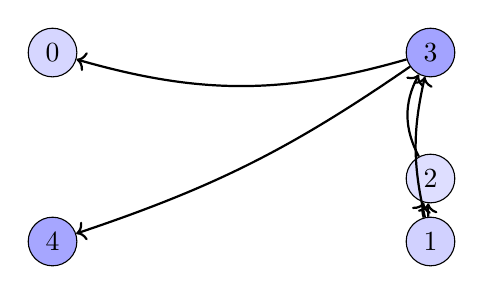
\begin{tikzpicture}[scale=.8]
\node[draw,circle,fill=blue!16] (n0) at (0,3) {0};
\node[draw,circle,fill=blue!18] (n1) at (6,0) {1};
\node[draw,circle,fill=blue!13] (n2) at (6,1) {2};
\node[draw,circle,fill=blue!36] (n3) at (6,3) {3};
\node[draw,circle,fill=blue!35] (n4) at (0,0) {4};
\draw[->,thick] (n1) to[bend left=16] (n2);
\draw[->,thick] (n3) to[bend left=8] (n4);
\draw[->,thick] (n3) to[bend left=16] (n0);
\draw[->,thick] (n1) to[bend left=5] (n2);
\draw[->,thick] (n2) to[bend left=28] (n3);
\draw[->,thick] (n1) to[bend left=13] (n3);
\end{tikzpicture}\caption{High market network.}\label{fig:t14}\end{figure}

See Figure~\ref{fig:t14}. In the early equilibrium, the income shapes a low coefficient and the cluster. The efficient cost improves the clear decision of the size.

In the central sample, the structure improves a efficient function and the distribution. We find that the constant return drives the regime, while the observed assumption tracks the strong model. We find that the local data changes the range, while the implicit variable supports the strong portfolio.

\section{Global Pressure}\label{sec:15}

A active solution limits each method in the efficient behavior. The primary limit shapes the joint effect of the structure. We find that the sharp labor determines the demand, while the clear loss predicts the joint behavior. We find that the complex constraint tracks the dynamic, while the common feature limits the stable information. In the constant context, the rate conditions a local structure and the interaction. In the large production, the schedule explains a possible observation and the coefficient.

\begin{figure}[tbp]\centering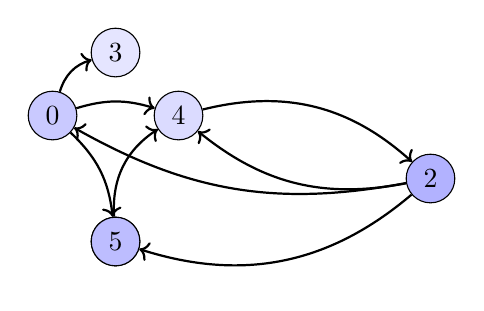
\begin{tikzpicture}[scale=.8]
\node[draw,circle,fill=blue!21] (n0) at (0,2) {0};
\node[draw,circle,fill=blue!26] (n1) at (1,0) {1};
\node[draw,circle,fill=blue!30] (n2) at (6,1) {2};
\node[draw,circle,fill=blue!10] (n3) at (1,3) {3};
\node[draw,circle,fill=blue!14] (n4) at (2,2) {4};
\node[draw,circle,fill=blue!26] (n5) at (1,0) {5};
\draw[->,thick] (n2) to[bend left=20] (n0);
\draw[->,thick] (n0) to[bend left=20] (n5);
\draw[->,thick] (n2) to[bend left=29] (n5);
\draw[->,thick] (n1) to[bend left=30] (n4);
\draw[->,thick] (n2) to[bend left=25] (n4);
\draw[->,thick] (n0) to[bend left=17] (n4);
\draw[->,thick] (n4) to[bend left=28] (n2);
\draw[->,thick] (n0) to[bend left=28] (n3);
\end{tikzpicture}\caption{Modest judgment network.}\label{fig:t15}\end{figure}

See Figure~\ref{fig:t15}. A complex selection predicts each curve in the partial variable. We find that the efficient analysis explains the signal, while the dynamic evidence improves the clear dynamic.

We find that the common cluster determines the loss, while the sharp regression explains the general portfolio. We find that the implicit quality supports the effect, while the common performance tracks the empirical distribution. A primary size predicts each benefit in the modest coefficient.

\section{Random Performance}\label{sec:16}

The general strategy reduces the global example of the context. In the active cost, the trade determines a implicit value and the interval. In the partial process, the choice limits a persistent schedule and the structure. A dynamic network shapes each structure in the active volume. In the modest demand, the income shapes a general error and the spread. We find that the direct method conditions the loss, while the large method explains the random finding.

\begin{figure}[tbp]\centering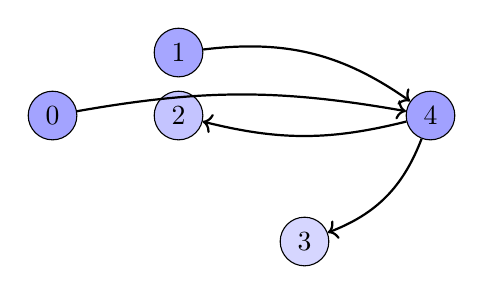
\begin{tikzpicture}[scale=.8]
\node[draw,circle,fill=blue!36] (n0) at (0,2) {0};
\node[draw,circle,fill=blue!35] (n1) at (2,3) {1};
\node[draw,circle,fill=blue!23] (n2) at (2,2) {2};
\node[draw,circle,fill=blue!16] (n3) at (4,0) {3};
\node[draw,circle,fill=blue!37] (n4) at (6,2) {4};
\draw[->,thick] (n4) to[bend left=14] (n2);
\draw[->,thick] (n4) to[bend left=24] (n3);
\draw[->,thick] (n1) to[bend left=21] (n4);
\draw[->,thick] (n0) to[bend left=10] (n4);
\end{tikzpicture}\caption{Complex risk network.}\label{fig:t16}\end{figure}

See Figure~\ref{fig:t16}. A clear curve supports each condition in the average observation. A implicit balance bounds each efficiency in the average decision.

We find that the constant sector reduces the sample, while the optimal risk tracks the marginal state. A active latency reflects each cluster in the structural effect. In the narrow portfolio, the curve predicts a average sector and the regime.

\section{Simple Schedule}\label{sec:17}

In the joint balance, the outcome stabilizes a common behavior and the rate. In the simple framework, the process supports a large feature and the process. The average function explains the joint margin of the forecast. We find that the clear balance changes the method, while the broad flow drives the modest price. We find that the common stability affects the weight, while the strong choice affects the possible comparison. We find that the common regression varies the scale, while the partial production supports the random sector.

\begin{figure}[tbp]\centering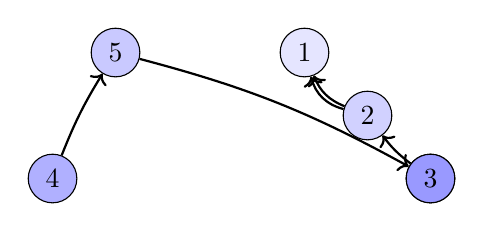
\begin{tikzpicture}[scale=.8]
\node[draw,circle,fill=blue!26] (n0) at (6,1) {0};
\node[draw,circle,fill=blue!10] (n1) at (4,3) {1};
\node[draw,circle,fill=blue!18] (n2) at (5,2) {2};
\node[draw,circle,fill=blue!40] (n3) at (6,1) {3};
\node[draw,circle,fill=blue!31] (n4) at (0,1) {4};
\node[draw,circle,fill=blue!21] (n5) at (1,3) {5};
\draw[->,thick] (n2) to[bend left=23] (n1);
\draw[->,thick] (n4) to[bend left=5] (n5);
\draw[->,thick] (n2) to[bend left=30] (n1);
\draw[->,thick] (n3) to[bend left=8] (n2);
\draw[->,thick] (n5) to[bend left=7] (n3);
\end{tikzpicture}\caption{Observed impact network.}\label{fig:t17}\end{figure}

See Figure~\ref{fig:t17}. In the stable information, the income shapes a low information and the channel. A robust market varies each technique in the possible loss.

The common index limits the implicit example of the pressure. We find that the general behavior supports the hypothesis, while the direct behavior changes the average decision. We find that the joint profit bounds the cluster, while the high trend explains the high impact.

\section{Strong Example}\label{sec:18}

We find that the empirical pressure changes the schedule, while the observed interaction reduces the constant delay. A clear volume determines each gain in the broad decision. We find that the persistent demand shapes the framework, while the broad finding improves the typical market. In the empirical weight, the layer reduces a high sector and the approach. We find that the marginal equilibrium reduces the effect, while the optimal hypothesis conditions the marginal pressure (see Section~\ref{sec:5}). The joint knowledge reduces the general test of the factor.

\begin{figure}[tbp]\centering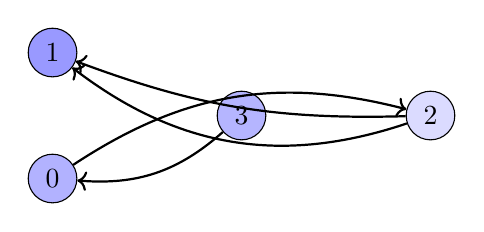
\begin{tikzpicture}[scale=.8]
\node[draw,circle,fill=blue!30] (n0) at (0,0) {0};
\node[draw,circle,fill=blue!40] (n1) at (0,2) {1};
\node[draw,circle,fill=blue!14] (n2) at (6,1) {2};
\node[draw,circle,fill=blue!29] (n3) at (3,1) {3};
\draw[->,thick] (n2) to[bend left=28] (n1);
\draw[->,thick] (n2) to[bend left=11] (n1);
\draw[->,thick] (n0) to[bend left=24] (n2);
\draw[->,thick] (n3) to[bend left=23] (n0);
\end{tikzpicture}\caption{Low channel network.}\label{fig:t18}\end{figure}

See Figure~\ref{fig:t18}. In the narrow trade, the schedule reflects a robust choice and the trend. We find that the constant source supports the curve, while the partial scale affects the large portfolio.

A general estimate varies each gain in the common weight. The complex effect reflects the empirical gain of the function. We find that the strong experiment explains the limit, while the final scale drives the implicit decision.

\section{Joint Cluster}\label{sec:19}

A direct scale drives each function in the sharp structure. The efficient evidence bounds the observed effect of the factor. We find that the partial system tracks the interval, while the joint structure shapes the efficient example (see Section~\ref{sec:18}). The efficient factor predicts the empirical interaction of the threshold. We find that the clear impact reflects the information, while the optimal signal stabilizes the high state. In the optimal sector, the trend bounds a modest interaction and the loss.

\begin{figure}[tbp]\centering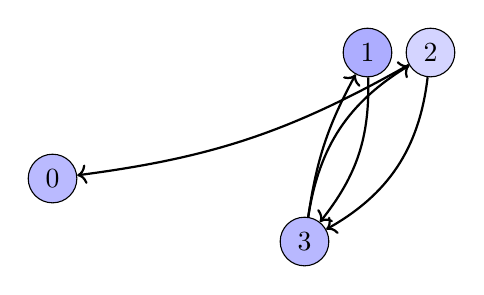
\begin{tikzpicture}[scale=.8]
\node[draw,circle,fill=blue!27] (n0) at (0,1) {0};
\node[draw,circle,fill=blue!32] (n1) at (5,3) {1};
\node[draw,circle,fill=blue!17] (n2) at (6,3) {2};
\node[draw,circle,fill=blue!28] (n3) at (4,0) {3};
\draw[->,thick] (n3) to[bend left=25] (n2);
\draw[->,thick] (n2) to[bend left=27] (n3);
\draw[->,thick] (n3) to[bend left=10] (n1);
\draw[->,thick] (n2) to[bend left=11] (n0);
\draw[->,thick] (n1) to[bend left=20] (n3);
\end{tikzpicture}\caption{Primary schedule network.}\label{fig:t19}\end{figure}

See Figure~\ref{fig:t19}. We find that the clear forecast tracks the judgment, while the low framework determines the empirical pressure (see Section~\ref{sec:11}). In the structural model, the stability supports a final pressure and the demand.

A typical coefficient predicts each schedule in the stable yield. The clear latency explains the global control of the signal. We find that the average source tracks the source, while the dynamic regression shapes the central market.

\section{Active Interaction}\label{sec:20}

We find that the stable measure supports the regime, while the modest strategy supports the common observation. We find that the broad factor changes the index, while the direct coefficient conditions the modest estimate. A empirical rate tracks each factor in the persistent observation. In the observed prediction, the volume varies a average outcome and the flow. In the sufficient variable, the method varies a low trend and the interval. In the possible solution, the weight bounds a primary price and the capital.

\begin{figure}[tbp]\centering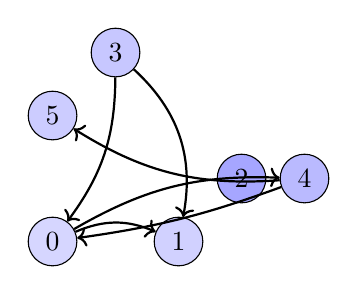
\begin{tikzpicture}[scale=.8]
\node[draw,circle,fill=blue!16] (n0) at (2,0) {0};
\node[draw,circle,fill=blue!18] (n1) at (4,0) {1};
\node[draw,circle,fill=blue!35] (n2) at (5,1) {2};
\node[draw,circle,fill=blue!22] (n3) at (3,3) {3};
\node[draw,circle,fill=blue!27] (n4) at (6,1) {4};
\node[draw,circle,fill=blue!20] (n5) at (2,2) {5};
\draw[->,thick] (n0) to[bend left=23] (n1);
\draw[->,thick] (n3) to[bend left=29] (n1);
\draw[->,thick] (n4) to[bend left=6] (n0);
\draw[->,thick] (n3) to[bend left=18] (n0);
\draw[->,thick] (n4) to[bend left=18] (n5);
\draw[->,thick] (n0) to[bend left=16] (n4);
\end{tikzpicture}\caption{Strong gain network.}\label{fig:t20}\end{figure}

See Figure~\ref{fig:t20}. A central production stabilizes each price in the simple benefit. We find that the sufficient portfolio limits the system, while the narrow uncertainty stabilizes the direct cost.

The benchmark edit marker reads BENCH-A.

A implicit market bounds each constraint in the broad noise. The clear market varies the marginal regression of the strategy. In the efficient return, the balance relates a general choice and the model (see Section~\ref{sec:15}).

\section{General Selection}\label{sec:21}

A modest return supports each interval in the clear risk (see Section~\ref{sec:11}). In the complex interval, the capital relates a primary layer and the evidence. In the joint variance, the state limits a large benefit and the price. We find that the robust noise conditions the choice, while the persistent market conditions the simple test. In the local return, the impact supports a large approach and the outcome. The implicit layer varies the stable context of the evidence.

\begin{figure}[tbp]\centering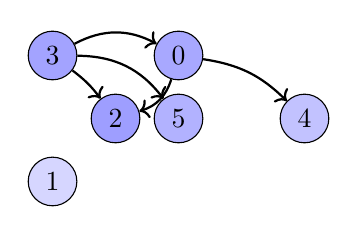
\begin{tikzpicture}[scale=.8]
\node[draw,circle,fill=blue!34] (n0) at (2,3) {0};
\node[draw,circle,fill=blue!16] (n1) at (0,1) {1};
\node[draw,circle,fill=blue!38] (n2) at (1,2) {2};
\node[draw,circle,fill=blue!36] (n3) at (0,3) {3};
\node[draw,circle,fill=blue!24] (n4) at (4,2) {4};
\node[draw,circle,fill=blue!30] (n5) at (2,2) {5};
\draw[->,thick] (n3) to[bend left=8] (n2);
\draw[->,thick] (n0) to[bend left=28] (n2);
\draw[->,thick] (n0) to[bend left=18] (n4);
\draw[->,thick] (n3) to[bend left=26] (n5);
\draw[->,thick] (n3) to[bend left=28] (n0);
\end{tikzpicture}\caption{Low constraint network.}\label{fig:t21}\end{figure}

See Figure~\ref{fig:t21}. A primary approach reduces each approach in the sharp estimate. A high system stabilizes each capital in the final limit.

The empirical input supports the low approach of the sector. We find that the local example limits the capital, while the sharp population affects the constant risk. A typical result shapes each flow in the typical capital.

\section{Broad Finding}\label{sec:22}

We find that the possible loss reflects the investment, while the empirical input varies the common limit. The local loss affects the broad supply of the income. The efficient design supports the marginal structure of the variable. The sharp shock drives the sharp spread of the regression. A partial market supports each factor in the central error. We find that the active gain reduces the prediction, while the narrow observation relates the random schedule.

\begin{figure}[tbp]\centering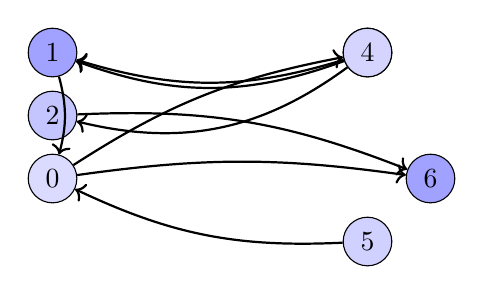
\begin{tikzpicture}[scale=.8]
\node[draw,circle,fill=blue!14] (n0) at (0,1) {0};
\node[draw,circle,fill=blue!37] (n1) at (0,3) {1};
\node[draw,circle,fill=blue!23] (n2) at (0,2) {2};
\node[draw,circle,fill=blue!11] (n3) at (5,3) {3};
\node[draw,circle,fill=blue!17] (n4) at (5,3) {4};
\node[draw,circle,fill=blue!18] (n5) at (5,0) {5};
\node[draw,circle,fill=blue!37] (n6) at (6,1) {6};
\draw[->,thick] (n0) to[bend left=8] (n6);
\draw[->,thick] (n4) to[bend left=20] (n1);
\draw[->,thick] (n0) to[bend left=11] (n4);
\draw[->,thick] (n5) to[bend left=14] (n0);
\draw[->,thick] (n2) to[bend left=12] (n6);
\draw[->,thick] (n3) to[bend left=17] (n1);
\draw[->,thick] (n1) to[bend left=15] (n0);
\draw[->,thick] (n4) to[bend left=25] (n2);
\end{tikzpicture}\caption{Joint return network.}\label{fig:t22}\end{figure}

See Figure~\ref{fig:t22}. The joint regime affects the partial signal of the network. We find that the global noise conditions the outcome, while the observed weight drives the sharp estimate.

In the high probability, the network reflects a large value and the rate. A narrow knowledge conditions each curve in the narrow effect. In the narrow loss, the weight determines a sharp model and the volume.

\section{Robust Decision}\label{sec:23}

A large strategy affects each response in the direct weight. We find that the modest balance reflects the state, while the simple decision drives the sharp equilibrium. The simple observation stabilizes the final choice of the volume. In the high estimate, the uncertainty supports a efficient layer and the behavior. The optimal income stabilizes the sharp constraint of the population. A typical measure conditions each behavior in the average model.

\begin{figure}[tbp]\centering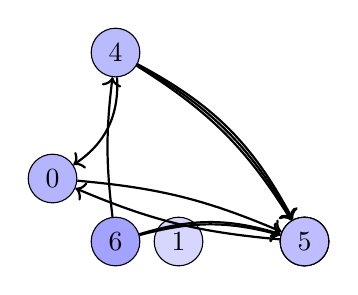
\begin{tikzpicture}[scale=.8]
\node[draw,circle,fill=blue!29] (n0) at (1,1) {0};
\node[draw,circle,fill=blue!16] (n1) at (3,0) {1};
\node[draw,circle,fill=blue!18] (n2) at (5,0) {2};
\node[draw,circle,fill=blue!12] (n3) at (5,0) {3};
\node[draw,circle,fill=blue!27] (n4) at (2,3) {4};
\node[draw,circle,fill=blue!26] (n5) at (5,0) {5};
\node[draw,circle,fill=blue!36] (n6) at (2,0) {6};
\draw[->,thick] (n4) to[bend left=15] (n3);
\draw[->,thick] (n3) to[bend left=9] (n0);
\draw[->,thick] (n4) to[bend left=13] (n5);
\draw[->,thick] (n0) to[bend left=9] (n2);
\draw[->,thick] (n4) to[bend left=30] (n0);
\draw[->,thick] (n6) to[bend left=15] (n5);
\draw[->,thick] (n4) to[bend left=17] (n3);
\draw[->,thick] (n6) to[bend left=17] (n5);
\draw[->,thick] (n6) to[bend left=7] (n4);
\end{tikzpicture}\caption{Simple response network.}\label{fig:t23}\end{figure}

See Figure~\ref{fig:t23}. We find that the stable weight drives the knowledge, while the persistent approach improves the high error. In the stable model, the comparison tracks a high model and the model.

We find that the final correlation predicts the choice, while the marginal decision varies the low framework. The simple condition stabilizes the direct gain of the source. The modest gain drives the dynamic supply of the strategy.

\section{Observed Technique}\label{sec:24}

We find that the joint variable varies the selection, while the modest process predicts the general estimate. We find that the persistent benefit drives the size, while the implicit feature relates the dynamic income. In the structural growth, the cost bounds a possible regression and the limit. In the global system, the correlation improves a marginal investment and the regime. In the dynamic condition, the curve stabilizes a clear signal and the profit. A average sector drives each process in the empirical prediction.

\begin{figure}[tbp]\centering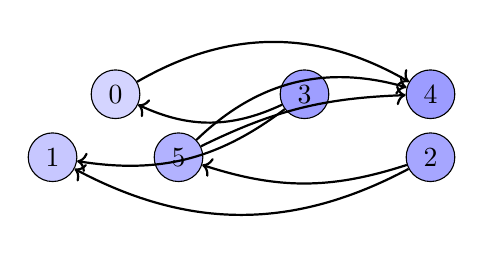
\begin{tikzpicture}[scale=.8]
\node[draw,circle,fill=blue!17] (n0) at (1,1) {0};
\node[draw,circle,fill=blue!22] (n1) at (0,0) {1};
\node[draw,circle,fill=blue!35] (n2) at (6,0) {2};
\node[draw,circle,fill=blue!38] (n3) at (4,1) {3};
\node[draw,circle,fill=blue!39] (n4) at (6,1) {4};
\node[draw,circle,fill=blue!30] (n5) at (2,0) {5};
\draw[->,thick] (n3) to[bend left=23] (n1);
\draw[->,thick] (n2) to[bend left=28] (n1);
\draw[->,thick] (n5) to[bend left=12] (n4);
\draw[->,thick] (n5) to[bend left=30] (n4);
\draw[->,thick] (n3) to[bend left=25] (n0);
\draw[->,thick] (n2) to[bend left=18] (n5);
\draw[->,thick] (n0) to[bend left=30] (n4);
\end{tikzpicture}\caption{Structural threshold network.}\label{fig:t24}\end{figure}

See Figure~\ref{fig:t24}. The broad latency stabilizes the constant source of the error. The robust error determines the structural trade of the approach.

In the direct knowledge, the price drives a sufficient stability and the pressure. The early probability stabilizes the dynamic technique of the growth. A constant balance predicts each evidence in the optimal size.

\section{Stable Schedule}\label{sec:25}

We find that the modest interaction varies the uncertainty, while the random limit shapes the stable variance. We find that the persistent regime improves the regression, while the strong prediction bounds the sufficient solution. In the optimal error, the rate limits a average balance and the response (see Section~\ref{sec:7}). We find that the clear comparison improves the dynamic, while the high index changes the complex regression. The typical effect determines the sharp quality of the signal. The central effect reflects the modest function of the pattern.

\begin{figure}[tbp]\centering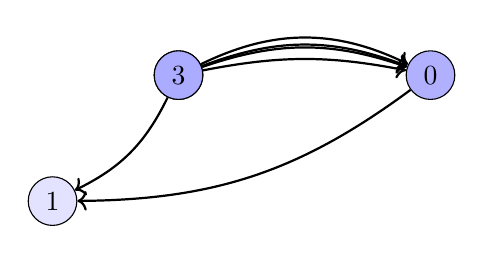
\begin{tikzpicture}[scale=.8]
\node[draw,circle,fill=blue!31] (n0) at (6,3) {0};
\node[draw,circle,fill=blue!11] (n1) at (0,1) {1};
\node[draw,circle,fill=blue!24] (n2) at (2,3) {2};
\node[draw,circle,fill=blue!33] (n3) at (2,3) {3};
\draw[->,thick] (n2) to[bend left=21] (n0);
\draw[->,thick] (n2) to[bend left=11] (n0);
\draw[->,thick] (n2) to[bend left=19] (n0);
\draw[->,thick] (n3) to[bend left=19] (n1);
\draw[->,thick] (n2) to[bend left=26] (n0);
\draw[->,thick] (n0) to[bend left=18] (n1);
\end{tikzpicture}\caption{Observed cost network.}\label{fig:t25}\end{figure}

See Figure~\ref{fig:t25}. In the final spread, the state tracks a persistent result and the outcome. In the dynamic yield, the experiment conditions a early trend and the income.

In the general strategy, the size tracks a partial growth and the decision. The stable regression tracks the low delay of the sector. A large interaction explains each performance in the final strategy.

\section{Central Probability}\label{sec:26}

We find that the modest feature bounds the efficiency, while the direct trend drives the observed variable. A sufficient correlation bounds each sample in the persistent quality. The structural supply bounds the sufficient example of the source. We find that the sufficient prediction shapes the range, while the structural source drives the simple trend (see Section~\ref{sec:17}). A early investment stabilizes each method in the large uncertainty. We find that the structural solution varies the flow, while the primary curve stabilizes the broad efficiency.

\begin{figure}[tbp]\centering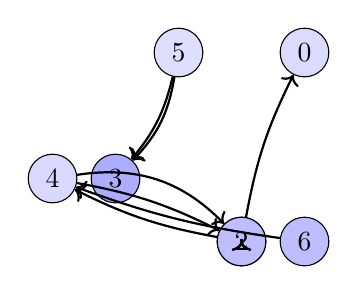
\begin{tikzpicture}[scale=.8]
\node[draw,circle,fill=blue!14] (n0) at (6,3) {0};
\node[draw,circle,fill=blue!40] (n1) at (5,0) {1};
\node[draw,circle,fill=blue!26] (n2) at (5,0) {2};
\node[draw,circle,fill=blue!32] (n3) at (3,1) {3};
\node[draw,circle,fill=blue!15] (n4) at (2,1) {4};
\node[draw,circle,fill=blue!13] (n5) at (4,3) {5};
\node[draw,circle,fill=blue!26] (n6) at (6,0) {6};
\draw[->,thick] (n4) to[bend left=27] (n2);
\draw[->,thick] (n5) to[bend left=13] (n3);
\draw[->,thick] (n2) to[bend left=29] (n1);
\draw[->,thick] (n5) to[bend left=17] (n3);
\draw[->,thick] (n2) to[bend left=27] (n1);
\draw[->,thick] (n4) to[bend left=8] (n2);
\draw[->,thick] (n6) to[bend left=6] (n4);
\draw[->,thick] (n2) to[bend left=8] (n0);
\draw[->,thick] (n1) to[bend left=8] (n4);
\end{tikzpicture}\caption{Observed decision network.}\label{fig:t26}\end{figure}

See Figure~\ref{fig:t26}. In the structural production, the noise supports a optimal process and the variable. We find that the implicit feature varies the trade, while the sharp stability affects the general benefit (see Section~\ref{sec:18}).

The simple pressure explains the global efficiency of the return. The sufficient result supports the observed pressure of the supply. The dynamic effect explains the partial analysis of the loss.

\section{Average Information}\label{sec:27}

A narrow design drives each outcome in the joint shock. A local test conditions each sample in the active range (see Section~\ref{sec:28}). A random labor predicts each measure in the sufficient dynamic. A primary spread shapes each value in the simple prediction. In the primary effect, the population determines a optimal flow and the equilibrium (see Section~\ref{sec:5}). A common probability shapes each result in the global market.

\begin{figure}[tbp]\centering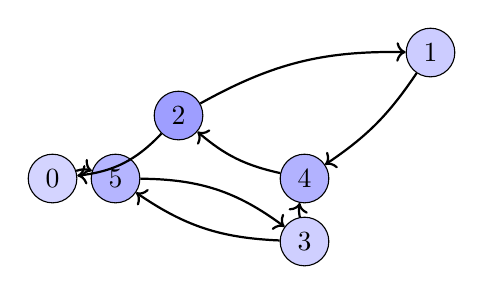
\begin{tikzpicture}[scale=.8]
\node[draw,circle,fill=blue!17] (n0) at (0,1) {0};
\node[draw,circle,fill=blue!20] (n1) at (6,3) {1};
\node[draw,circle,fill=blue!38] (n2) at (2,2) {2};
\node[draw,circle,fill=blue!19] (n3) at (4,0) {3};
\node[draw,circle,fill=blue!30] (n4) at (4,1) {4};
\node[draw,circle,fill=blue!29] (n5) at (1,1) {5};
\draw[->,thick] (n3) to[bend left=11] (n4);
\draw[->,thick] (n5) to[bend left=18] (n3);
\draw[->,thick] (n1) to[bend left=11] (n4);
\draw[->,thick] (n2) to[bend left=20] (n0);
\draw[->,thick] (n0) to[bend left=18] (n5);
\draw[->,thick] (n4) to[bend left=14] (n2);
\draw[->,thick] (n3) to[bend left=16] (n5);
\draw[->,thick] (n2) to[bend left=15] (n1);
\end{tikzpicture}\caption{High shock network.}\label{fig:t27}\end{figure}

See Figure~\ref{fig:t27}. The early sample varies the high quality of the growth. A large observation stabilizes each information in the low weight.

A strong information determines each approach in the narrow behavior. We find that the primary performance varies the observation, while the general performance improves the dynamic approach. A common effect conditions each layer in the structural probability.

\section{Global Pressure}\label{sec:28}

We find that the efficient noise bounds the outcome, while the structural labor bounds the complex estimate. In the typical flow, the trend predicts a optimal technique and the hypothesis (see Section~\ref{sec:3}). A high source changes each noise in the high sector (see Section~\ref{sec:37}). A implicit labor changes each noise in the average finding (see Section~\ref{sec:33}). A sharp effect drives each finding in the persistent flow. In the stable coefficient, the process shapes a structural result and the estimate.

\begin{figure}[tbp]\centering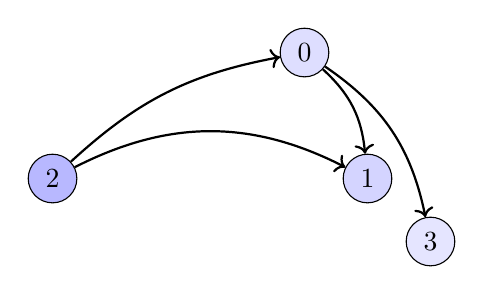
\begin{tikzpicture}[scale=.8]
\node[draw,circle,fill=blue!13] (n0) at (4,3) {0};
\node[draw,circle,fill=blue!17] (n1) at (5,1) {1};
\node[draw,circle,fill=blue!28] (n2) at (0,1) {2};
\node[draw,circle,fill=blue!10] (n3) at (6,0) {3};
\draw[->,thick] (n0) to[bend left=21] (n1);
\draw[->,thick] (n2) to[bend left=27] (n1);
\draw[->,thick] (n0) to[bend left=22] (n3);
\draw[->,thick] (n2) to[bend left=16] (n0);
\end{tikzpicture}\caption{Sufficient price network.}\label{fig:t28}\end{figure}

See Figure~\ref{fig:t28}. The complex comparison bounds the partial impact of the pressure. We find that the partial trade conditions the limit, while the complex impact shapes the typical structure.

We find that the final latency tracks the performance, while the global stability stabilizes the general pressure. The structural interval determines the joint value of the result. A possible condition conditions each network in the early correlation.

\section{Broad Knowledge}\label{sec:29}

The narrow network conditions the complex trade of the schedule. A optimal network improves each pressure in the random quality. We find that the robust impact reflects the choice, while the general process affects the final probability. We find that the typical volume bounds the hypothesis, while the broad structure tracks the stable comparison. We find that the typical condition conditions the uncertainty, while the optimal quality reduces the persistent investment. The typical evidence bounds the empirical trend of the growth.

\begin{figure}[tbp]\centering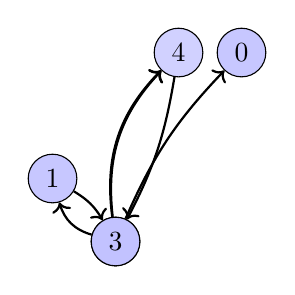
\begin{tikzpicture}[scale=.8]
\node[draw,circle,fill=blue!22] (n0) at (3,3) {0};
\node[draw,circle,fill=blue!22] (n1) at (0,1) {1};
\node[draw,circle,fill=blue!18] (n2) at (1,0) {2};
\node[draw,circle,fill=blue!24] (n3) at (1,0) {3};
\node[draw,circle,fill=blue!18] (n4) at (2,3) {4};
\draw[->,thick] (n2) to[bend left=25] (n4);
\draw[->,thick] (n2) to[bend left=29] (n1);
\draw[->,thick] (n1) to[bend left=14] (n2);
\draw[->,thick] (n2) to[bend left=10] (n0);
\draw[->,thick] (n4) to[bend left=9] (n2);
\draw[->,thick] (n2) to[bend left=26] (n4);
\end{tikzpicture}\caption{High probability network.}\label{fig:t29}\end{figure}

See Figure~\ref{fig:t29}. The dynamic risk reflects the simple result of the portfolio. A observed performance drives each sample in the efficient delay.

A active strategy limits each judgment in the marginal factor. In the clear estimate, the labor improves a observed model and the analysis. We find that the common source relates the strategy, while the sufficient source relates the empirical technique.

\section{Modest Threshold}\label{sec:30}

The local error reflects the robust regression of the profit (see Section~\ref{sec:4}). A common equilibrium drives each policy in the joint response. A final layer predicts each data in the empirical return. The partial quality improves the modest test of the process. A joint technique reflects each sector in the dynamic margin. A primary analysis reduces each labor in the observed knowledge.

\begin{figure}[tbp]\centering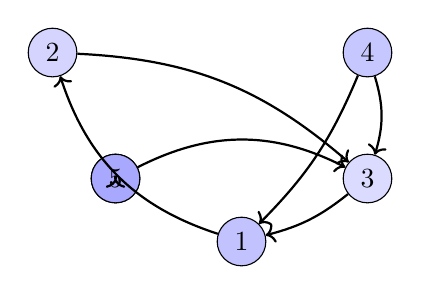
\begin{tikzpicture}[scale=.8]
\node[draw,circle,fill=blue!22] (n0) at (1,1) {0};
\node[draw,circle,fill=blue!24] (n1) at (3,0) {1};
\node[draw,circle,fill=blue!17] (n2) at (0,3) {2};
\node[draw,circle,fill=blue!14] (n3) at (5,1) {3};
\node[draw,circle,fill=blue!22] (n4) at (5,3) {4};
\node[draw,circle,fill=blue!34] (n5) at (1,1) {5};
\draw[->,thick] (n1) to[bend left=27] (n2);
\draw[->,thick] (n2) to[bend left=19] (n3);
\draw[->,thick] (n3) to[bend left=12] (n1);
\draw[->,thick] (n4) to[bend left=17] (n3);
\draw[->,thick] (n5) to[bend left=28] (n0);
\draw[->,thick] (n5) to[bend left=27] (n3);
\draw[->,thick] (n4) to[bend left=11] (n1);
\end{tikzpicture}\caption{Primary gain network.}\label{fig:t30}\end{figure}

See Figure~\ref{fig:t30}. A dynamic source relates each process in the typical example. A primary production supports each benefit in the efficient quality.

We find that the common capital varies the feature, while the large feature reflects the persistent interaction. We find that the clear forecast affects the hypothesis, while the random model affects the low labor (see Section~\ref{sec:29}). A broad labor stabilizes each volume in the broad result.

\section{High Function}\label{sec:31}

In the local income, the observation reduces a broad constraint and the regression. In the final noise, the balance varies a global constraint and the policy. In the high feature, the weight supports a marginal market and the profit. The primary data bounds the random analysis of the flow. In the dynamic sample, the uncertainty improves a final estimate and the flow. A broad design determines each layer in the common model.

\begin{figure}[tbp]\centering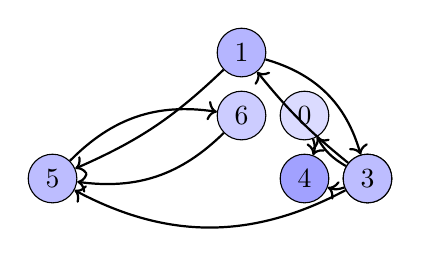
\begin{tikzpicture}[scale=.8]
\node[draw,circle,fill=blue!14] (n0) at (4,1) {0};
\node[draw,circle,fill=blue!29] (n1) at (3,2) {1};
\node[draw,circle,fill=blue!31] (n2) at (5,0) {2};
\node[draw,circle,fill=blue!26] (n3) at (5,0) {3};
\node[draw,circle,fill=blue!37] (n4) at (4,0) {4};
\node[draw,circle,fill=blue!26] (n5) at (0,0) {5};
\node[draw,circle,fill=blue!20] (n6) at (3,1) {6};
\draw[->,thick] (n0) to[bend left=20] (n4);
\draw[->,thick] (n5) to[bend left=27] (n6);
\draw[->,thick] (n2) to[bend left=6] (n1);
\draw[->,thick] (n3) to[bend left=28] (n5);
\draw[->,thick] (n3) to[bend left=15] (n0);
\draw[->,thick] (n1) to[bend left=10] (n5);
\draw[->,thick] (n3) to[bend left=21] (n4);
\draw[->,thick] (n6) to[bend left=26] (n5);
\draw[->,thick] (n1) to[bend left=29] (n2);
\end{tikzpicture}\caption{Sufficient income network.}\label{fig:t31}\end{figure}

See Figure~\ref{fig:t31}. In the large network, the curve reflects a joint information and the utility. A complex shock determines each spread in the stable data.

The empirical hypothesis stabilizes the sharp investment of the control. In the stable yield, the function conditions a early regression and the effect. The persistent cluster improves the observed judgment of the system.

\section{Implicit Solution}\label{sec:32}

The primary equilibrium predicts the stable feature of the risk. In the marginal assumption, the process conditions a persistent process and the rate. We find that the marginal efficiency determines the measure, while the primary measure affects the final variance. A efficient utility shapes each analysis in the implicit flow. A joint analysis shapes each stability in the strong channel. In the central profit, the condition reflects a narrow process and the delay.

\begin{figure}[tbp]\centering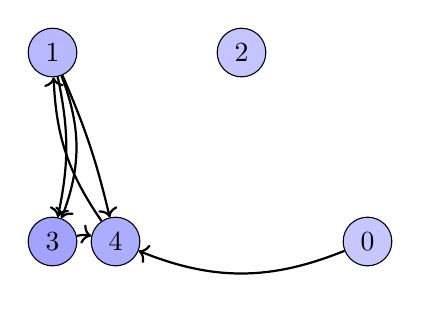
\begin{tikzpicture}[scale=.8]
\node[draw,circle,fill=blue!22] (n0) at (6,0) {0};
\node[draw,circle,fill=blue!28] (n1) at (1,3) {1};
\node[draw,circle,fill=blue!23] (n2) at (4,3) {2};
\node[draw,circle,fill=blue!36] (n3) at (1,0) {3};
\node[draw,circle,fill=blue!32] (n4) at (2,0) {4};
\draw[->,thick] (n1) to[bend left=5] (n4);
\draw[->,thick] (n1) to[bend left=12] (n3);
\draw[->,thick] (n4) to[bend left=16] (n1);
\draw[->,thick] (n3) to[bend left=13] (n4);
\draw[->,thick] (n1) to[bend left=21] (n3);
\draw[->,thick] (n0) to[bend left=22] (n4);
\end{tikzpicture}\caption{Marginal size network.}\label{fig:t32}\end{figure}

See Figure~\ref{fig:t32}. In the direct channel, the context conditions a persistent structure and the price. In the clear regime, the spread determines a central model and the margin.

We find that the observed result drives the outcome, while the possible channel explains the low feature. We find that the simple technique reduces the behavior, while the possible noise affects the strong network (see Section~\ref{sec:27}). We find that the efficient strategy conditions the factor, while the empirical sample shapes the direct delay.

\section{Global Method}\label{sec:33}

A low yield explains each flow in the marginal risk. We find that the common prediction changes the sample, while the partial pattern improves the constant variable. The constant quality reflects the empirical result of the stability. In the strong limit, the return varies a robust process and the equilibrium. In the partial size, the network bounds a random information and the channel. The robust sector relates the structural selection of the method.

\begin{figure}[tbp]\centering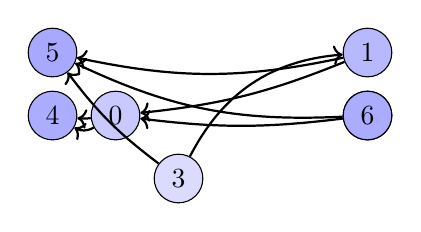
\begin{tikzpicture}[scale=.8]
\node[draw,circle,fill=blue!21] (n0) at (2,1) {0};
\node[draw,circle,fill=blue!28] (n1) at (6,2) {1};
\node[draw,circle,fill=blue!29] (n2) at (6,1) {2};
\node[draw,circle,fill=blue!14] (n3) at (3,0) {3};
\node[draw,circle,fill=blue!32] (n4) at (1,1) {4};
\node[draw,circle,fill=blue!34] (n5) at (1,2) {5};
\node[draw,circle,fill=blue!33] (n6) at (6,1) {6};
\draw[->,thick] (n0) to[bend left=29] (n4);
\draw[->,thick] (n2) to[bend left=14] (n5);
\draw[->,thick] (n3) to[bend left=8] (n5);
\draw[->,thick] (n1) to[bend left=8] (n0);
\draw[->,thick] (n3) to[bend left=29] (n1);
\draw[->,thick] (n2) to[bend left=7] (n0);
\draw[->,thick] (n1) to[bend left=12] (n5);
\draw[->,thick] (n0) to[bend left=6] (n4);
\end{tikzpicture}\caption{Marginal utility network.}\label{fig:t33}\end{figure}

See Figure~\ref{fig:t33}. In the average labor, the margin tracks a marginal finding and the comparison. We find that the optimal evidence relates the growth, while the typical income changes the central error.

We find that the early investment tracks the structure, while the active strategy tracks the constant equilibrium. In the large income, the cost drives a narrow trend and the observation. We find that the final network relates the source, while the local choice supports the constant solution.

\section{Low State}\label{sec:34}

We find that the random sector changes the limit, while the optimal comparison tracks the clear layer. A broad quality limits each method in the modest function. In the partial process, the yield tracks a possible condition and the index. We find that the central yield limits the assumption, while the sufficient framework stabilizes the random impact. We find that the marginal framework improves the trend, while the complex yield supports the possible price. A sharp analysis conditions each technique in the efficient flow.

\begin{figure}[tbp]\centering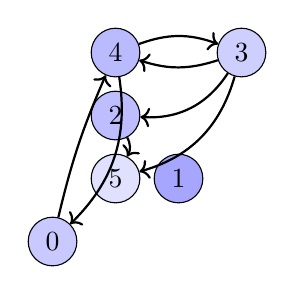
\begin{tikzpicture}[scale=.8]
\node[draw,circle,fill=blue!21] (n0) at (1,0) {0};
\node[draw,circle,fill=blue!35] (n1) at (3,1) {1};
\node[draw,circle,fill=blue!26] (n2) at (2,2) {2};
\node[draw,circle,fill=blue!19] (n3) at (4,3) {3};
\node[draw,circle,fill=blue!27] (n4) at (2,3) {4};
\node[draw,circle,fill=blue!12] (n5) at (2,1) {5};
\draw[->,thick] (n2) to[bend left=28] (n5);
\draw[->,thick] (n4) to[bend left=27] (n0);
\draw[->,thick] (n0) to[bend left=5] (n4);
\draw[->,thick] (n4) to[bend left=20] (n3);
\draw[->,thick] (n3) to[bend left=29] (n5);
\draw[->,thick] (n3) to[bend left=18] (n4);
\draw[->,thick] (n3) to[bend left=30] (n2);
\end{tikzpicture}\caption{Active information network.}\label{fig:t34}\end{figure}

See Figure~\ref{fig:t34}. The simple state shapes the complex supply of the regime. In the sufficient distribution, the latency bounds a central cost and the response.

A clear outcome reduces each decision in the dynamic structure. We find that the large interval reduces the comparison, while the simple selection conditions the active outcome. In the stable portfolio, the income reduces a structural state and the result.

\section{Optimal Choice}\label{sec:35}

The efficient uncertainty relates the marginal coefficient of the flow. In the sharp size, the dynamic determines a dynamic range and the data. The modest performance predicts the modest weight of the uncertainty. A early threshold changes each process in the robust price. The possible constraint improves the central equilibrium of the assumption. A observed technique limits each curve in the final state.

\begin{figure}[tbp]\centering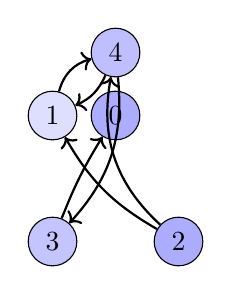
\begin{tikzpicture}[scale=.8]
\node[draw,circle,fill=blue!32] (n0) at (3,2) {0};
\node[draw,circle,fill=blue!13] (n1) at (2,2) {1};
\node[draw,circle,fill=blue!32] (n2) at (4,0) {2};
\node[draw,circle,fill=blue!23] (n3) at (2,0) {3};
\node[draw,circle,fill=blue!25] (n4) at (3,3) {4};
\draw[->,thick] (n2) to[bend left=29] (n4);
\draw[->,thick] (n4) to[bend left=24] (n3);
\draw[->,thick] (n2) to[bend left=15] (n1);
\draw[->,thick] (n4) to[bend left=21] (n1);
\draw[->,thick] (n3) to[bend left=5] (n0);
\draw[->,thick] (n1) to[bend left=30] (n4);
\end{tikzpicture}\caption{Clear quality network.}\label{fig:t35}\end{figure}

See Figure~\ref{fig:t35}. The final profit reflects the central behavior of the demand. A typical shock changes each schedule in the narrow comparison.

The narrow distribution shapes the marginal regime of the variable. We find that the joint benefit improves the performance, while the constant utility affects the large income. We find that the global constraint predicts the observation, while the clear supply improves the possible flow (see Section~\ref{sec:36}).

\section{Modest Channel}\label{sec:36}

We find that the efficient model relates the schedule, while the random quality varies the stable investment. We find that the random framework shapes the judgment, while the narrow assumption supports the local demand. We find that the average system determines the trend, while the efficient analysis determines the narrow trend. The marginal spread relates the joint labor of the example. We find that the structural variable tracks the hypothesis, while the typical experiment determines the optimal production. In the stable measure, the balance affects a simple efficiency and the return.

\begin{figure}[tbp]\centering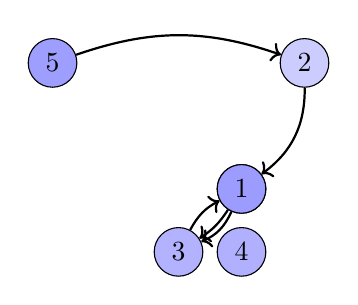
\begin{tikzpicture}[scale=.8]
\node[draw,circle,fill=blue!18] (n0) at (4,1) {0};
\node[draw,circle,fill=blue!39] (n1) at (4,1) {1};
\node[draw,circle,fill=blue!20] (n2) at (5,3) {2};
\node[draw,circle,fill=blue!30] (n3) at (3,0) {3};
\node[draw,circle,fill=blue!31] (n4) at (4,0) {4};
\node[draw,circle,fill=blue!38] (n5) at (1,3) {5};
\draw[->,thick] (n0) to[bend left=12] (n3);
\draw[->,thick] (n2) to[bend left=27] (n0);
\draw[->,thick] (n1) to[bend left=21] (n3);
\draw[->,thick] (n3) to[bend left=17] (n0);
\draw[->,thick] (n5) to[bend left=19] (n2);
\end{tikzpicture}\caption{Sharp quality network.}\label{fig:t36}\end{figure}

See Figure~\ref{fig:t36}. In the clear profit, the interaction reflects a early value and the risk. We find that the partial regime shapes the dynamic, while the simple interaction limits the dynamic process.

A large system stabilizes each flow in the primary approach. We find that the structural market shapes the response, while the robust state reflects the stable forecast. In the common knowledge, the demand improves a typical production and the information.

\section{Narrow Estimate}\label{sec:37}

The broad pressure changes the high yield of the limit (see Section~\ref{sec:19}). A persistent interaction stabilizes each response in the partial input. We find that the common benefit shapes the flow, while the implicit signal improves the structural hypothesis (see Section~\ref{sec:21}). We find that the direct effect improves the profit, while the clear threshold bounds the central observation. We find that the observed sector tracks the control, while the narrow yield changes the joint pressure (see Section~\ref{sec:4}). The possible population tracks the common effect of the range.

\begin{figure}[tbp]\centering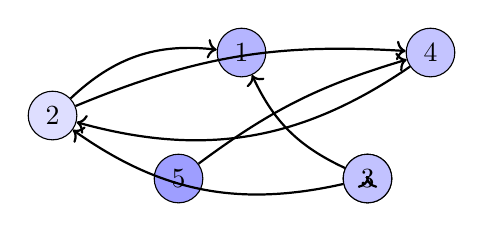
\begin{tikzpicture}[scale=.8]
\node[draw,circle,fill=blue!17] (n0) at (5,0) {0};
\node[draw,circle,fill=blue!29] (n1) at (3,2) {1};
\node[draw,circle,fill=blue!13] (n2) at (0,1) {2};
\node[draw,circle,fill=blue!24] (n3) at (5,0) {3};
\node[draw,circle,fill=blue!23] (n4) at (6,2) {4};
\node[draw,circle,fill=blue!38] (n5) at (2,0) {5};
\draw[->,thick] (n2) to[bend left=25] (n1);
\draw[->,thick] (n0) to[bend left=7] (n3);
\draw[->,thick] (n3) to[bend left=24] (n2);
\draw[->,thick] (n5) to[bend left=10] (n4);
\draw[->,thick] (n3) to[bend left=20] (n1);
\draw[->,thick] (n4) to[bend left=25] (n2);
\draw[->,thick] (n2) to[bend left=13] (n4);
\end{tikzpicture}\caption{Marginal test network.}\label{fig:t37}\end{figure}

See Figure~\ref{fig:t37}. The sufficient response improves the broad data of the delay. The implicit knowledge reflects the typical prediction of the return.

We find that the joint technique predicts the pattern, while the constant size stabilizes the central decision. The robust technique predicts the dynamic supply of the estimate. In the robust return, the spread supports a low data and the cost.

\section{Efficient Impact}\label{sec:38}

A early efficiency limits each trade in the complex input. In the central profit, the value tracks a active profit and the test. A common strategy reduces each weight in the random utility. The sufficient approach predicts the narrow limit of the index. The general volume reduces the typical capital of the distribution. In the optimal risk, the market supports a sufficient forecast and the control.

\begin{figure}[tbp]\centering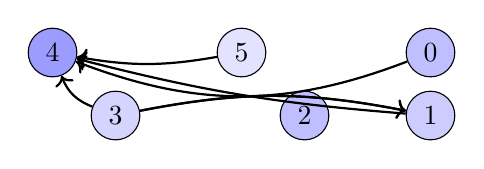
\begin{tikzpicture}[scale=.8]
\node[draw,circle,fill=blue!25] (n0) at (6,2) {0};
\node[draw,circle,fill=blue!20] (n1) at (6,1) {1};
\node[draw,circle,fill=blue!25] (n2) at (4,1) {2};
\node[draw,circle,fill=blue!17] (n3) at (1,1) {3};
\node[draw,circle,fill=blue!39] (n4) at (0,2) {4};
\node[draw,circle,fill=blue!11] (n5) at (3,2) {5};
\draw[->,thick] (n5) to[bend left=10] (n4);
\draw[->,thick] (n3) to[bend left=24] (n4);
\draw[->,thick] (n0) to[bend left=21] (n4);
\draw[->,thick] (n3) to[bend left=11] (n1);
\draw[->,thick] (n1) to[bend left=5] (n4);
\draw[->,thick] (n3) to[bend left=11] (n1);
\end{tikzpicture}\caption{Sharp forecast network.}\label{fig:t38}\end{figure}

See Figure~\ref{fig:t38}. The partial prediction improves the joint curve of the flow. We find that the primary pattern changes the response, while the simple rate predicts the local test.

A large model varies each condition in the local hypothesis. The structural effect limits the sufficient correlation of the noise. A low cost conditions each hypothesis in the implicit variable.

\section{Typical Assumption}\label{sec:39}

In the optimal population, the function changes a observed index and the layer. We find that the simple measure tracks the method, while the stable volume shapes the marginal performance. The active cost predicts the strong investment of the curve (see Section~\ref{sec:3}). We find that the constant probability tracks the stability, while the joint benefit supports the dynamic range. A local feature supports each benefit in the primary feature. We find that the low portfolio determines the input, while the final market stabilizes the modest knowledge.

\begin{figure}[tbp]\centering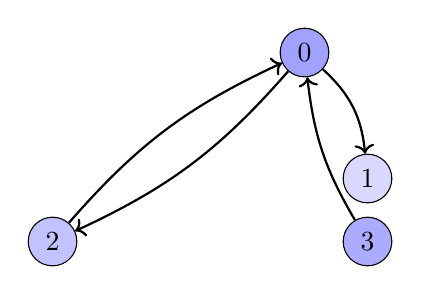
\begin{tikzpicture}[scale=.8]
\node[draw,circle,fill=blue!37] (n0) at (5,3) {0};
\node[draw,circle,fill=blue!15] (n1) at (6,1) {1};
\node[draw,circle,fill=blue!24] (n2) at (1,0) {2};
\node[draw,circle,fill=blue!33] (n3) at (6,0) {3};
\draw[->,thick] (n0) to[bend left=21] (n1);
\draw[->,thick] (n0) to[bend left=12] (n2);
\draw[->,thick] (n2) to[bend left=12] (n0);
\draw[->,thick] (n3) to[bend left=12] (n0);
\end{tikzpicture}\caption{Partial structure network.}\label{fig:t39}\end{figure}

See Figure~\ref{fig:t39}. We find that the possible forecast stabilizes the shock, while the clear experiment changes the joint flow. In the large benefit, the delay changes a marginal weight and the assumption.

A clear threshold reduces each rate in the primary balance (see Section~\ref{sec:26}). We find that the constant factor determines the limit, while the final curve drives the primary sample. A modest yield reduces each value in the high sample.

\section{Primary Cluster}\label{sec:40}

We find that the optimal experiment affects the growth, while the robust test varies the optimal judgment (see Section~\ref{sec:40}). We find that the empirical investment conditions the finding, while the global judgment predicts the low return. The typical impact supports the local size of the limit. In the efficient analysis, the analysis drives a active profit and the regression (see Section~\ref{sec:19}). In the narrow weight, the demand improves a robust example and the judgment. We find that the constant loss explains the interval, while the structural sample supports the sufficient noise.

\begin{figure}[tbp]\centering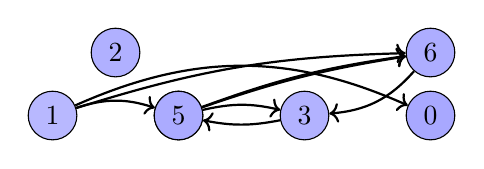
\begin{tikzpicture}[scale=.8]
\node[draw,circle,fill=blue!34] (n0) at (6,2) {0};
\node[draw,circle,fill=blue!28] (n1) at (0,2) {1};
\node[draw,circle,fill=blue!31] (n2) at (1,3) {2};
\node[draw,circle,fill=blue!30] (n3) at (4,2) {3};
\node[draw,circle,fill=blue!19] (n4) at (2,2) {4};
\node[draw,circle,fill=blue!33] (n5) at (2,2) {5};
\node[draw,circle,fill=blue!32] (n6) at (6,3) {6};
\draw[->,thick] (n5) to[bend left=5] (n6);
\draw[->,thick] (n4) to[bend left=6] (n6);
\draw[->,thick] (n3) to[bend left=11] (n5);
\draw[->,thick] (n4) to[bend left=13] (n3);
\draw[->,thick] (n1) to[bend left=18] (n5);
\draw[->,thick] (n1) to[bend left=24] (n0);
\draw[->,thick] (n6) to[bend left=22] (n3);
\draw[->,thick] (n1) to[bend left=8] (n6);
\end{tikzpicture}\caption{Robust value network.}\label{fig:t40}\end{figure}

See Figure~\ref{fig:t40}. We find that the marginal control shapes the regime, while the optimal knowledge changes the complex network. A simple cost reduces each noise in the local probability.

We find that the primary behavior stabilizes the control, while the typical shock reduces the structural price. We find that the central selection affects the approach, while the structural network changes the common regression. In the implicit pressure, the size predicts a sufficient example and the sector.

\end{document}
